\chapter{Scottsdale and the Operating Math of Wealth}

This School of Hard Knocks interview, curated by LazyingArt LLC, is less a chapter about celebrity wealth than a chapter about the operating math the host keeps extracting from wealthy operators once they finally talk. The lecture begins with spectacle---luxury cars, whispered tips, a billionaire who owns an NBA team, and a promised meeting with Robert Kiyosaki---but its real content lies in a sequence of local models: access under friction, scale under stress, time under a fixed budget, reinvestment under self-restraint, leverage through institutions, and sales through repeated rejection. No validated mathematical screenshots survived review for this episode, so the figures below are transcript-based reconstructions rather than redrawings of visible board work.

\section{Scottsdale as a Wealth Field}

\paragraph{Anecdote.} The lecture opens by showing us the payoff before it shows us the search. A bystander whispers that there is a billionaire inside. The host walks in, learns that the man owns the Phoenix Suns, and then, before the formal episode has properly begun, we also glimpse Robert Kiyosaki. The rhythm is intentional. We are first shown that genuine access is possible.

\paragraph{Claim.} Only after this cold open does the host widen the frame and tell us what the experiment is. Scottsdale is presented as one of the richest cities in America, a place with an unusually high concentration of millionaires and billionaires. Rolls Royce, McLaren, Bentley, valet stands, luxury restaurants, and private entrances are therefore not background decoration. They define the search geometry.

\paragraph{Mechanism.} The first mechanism is social rather than financial. Wealth is visible, but doctrine is guarded. The early encounters are refusals, partial refusals, short answers, and people who simply do not want to be on camera. The host's own rule is therefore important: every no is a step closer to a yes. We should preserve that line, because it gives the lecture its first piece of operating math. Before we ever arrive at leverage or reinvestment, we are made to see that access itself has a cost.

\section{From Refusal to Real Signal: The FinTech Bottleneck}

\paragraph{Anecdote.} After repeated rebuffs, the host finally persuades a private founder to speak by showing the scale of the channel and the record of earlier interviews. This is an important turn. The lecture moves from cold approaches to earned credibility. Only then does a private operator offer something like a usable business answer.

\paragraph{Claim.} The host asks the sharpest question in the first half of the lecture: what blocks the move from a \$10 million company to a \$100 million business? The point is not to collect another origin story. The point is to isolate the scale transition itself.

\begin{equation}
S_0 \approx \$10\,\text{million},\qquad S_1 \approx \$100\,\text{million},\qquad \frac{S_1}{S_0} \approx 10.
\end{equation}

We should keep the notation cautious. These are scale markers, not audited categories. But the tenfold jump is exactly the right way to frame the problem, because the founder's answer is not about inspiration or branding. It is about organizational readiness.

\paragraph{Mechanism.} The answer is that firms often address scale only when they have to. They do not build enough process or enough structure early; they wait until growth has already hit them. A clean reconstruction of the point is

\begin{equation}
\text{stress}_{\text{growth}} \propto \text{demand} - \text{prepared capacity}.
\end{equation}

If demand exceeds prepared capacity, growth appears as disorder. If capacity is built in advance, growth is absorbed rather than chased.

We may draw the contrast schematically:

\begin{figure}[h]
\centering
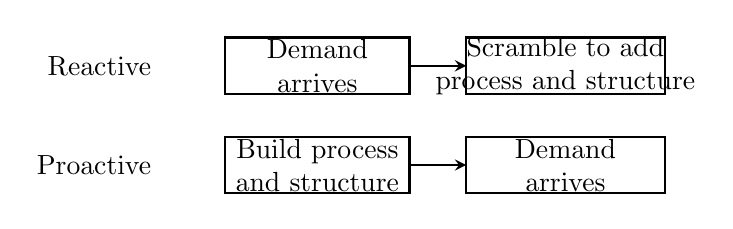
\begin{tikzpicture}[x=1cm,y=1cm,>=stealth,thick,scale=0.9]
\draw (-0.1,1.8) node[left]{Reactive};
\draw (-0.1,0.4) node[left]{Proactive};

\draw (0.8,1.4) rectangle (3.4,2.2) node[pos=.5,align=center]{Demand\\arrives};
\draw (4.2,1.4) rectangle (7.0,2.2) node[pos=.5,align=center]{Scramble to add\\process and structure};
\draw[->] (3.4,1.8) -- (4.2,1.8);

\draw (0.8,0.0) rectangle (3.4,0.8) node[pos=.5,align=center]{Build process\\and structure};
\draw (4.2,0.0) rectangle (7.0,0.8) node[pos=.5,align=center]{Demand\\arrives};
\draw[->] (3.4,0.4) -- (4.2,0.4);
\end{tikzpicture}
\end{figure}

The lower lane is the founder's doctrine: build the machine before the shock.

\subsection{Question \& Answer}

\paragraph{Question.} Why do companies choke when they try to scale?

\paragraph{Answer.} Because they confuse growth with reaction. The founder's phrase is that one must get out of one's own way. That sounds psychological, but in context it is organizational. Scale punishes firms that postpone structure until after demand arrives. The interview then widens the point from systems to management. A bad boss becomes instructive because he teaches by counterexample: do not hire talented people and then silence them; do not force arbitrary deadlines for the sake of ego; do not stop listening to customers and employees. By the time the founder adds that younger workers often jump ship after only \(12\) to \(16\) months, the lecture has already shifted from a revenue question to an institutional question. Scale is not merely more demand. Scale is more demand carried by durable organization.

The host's own recap after the interview is also worth preserving. He says the founder had reached the root of the customer problem: solve what people want and need, and wealth follows. This gives the section its final bridge. We begin with scale readiness, but the scale-ready firm still has to solve something real.

\section{Matt Ishbia and the Arithmetic of Time}

\paragraph{Anecdote.} The next whisper of access sends the host to another billionaire, and this time the surprise is even more useful. The owner of the Phoenix Suns did not make his money by founding a glamorous consumer technology platform. He says he spent his life in mortgages, building that business for more than twenty years.

\paragraph{Claim.} Ishbia gives the lecture two clean numerical anchors. First, the mortgage company grew from \(12\) people to \(9000\). Second, every person has \(24\) hours. The first number marks industrial scale. The second supplies the invariant against which human performance must be measured.

\begin{align}
N_0 &= 12,\qquad N_1 = 9000,\qquad \frac{N_1}{N_0} = 750,\\
T_{\text{day}} &= 24\ \mathrm{h},\qquad T_{\text{sleep}} \in \{8,6,5\}\ \mathrm{h}.
\end{align}

The lecture is now pushing against a common fantasy. One does not need a glamorous business category in order to build extraordinary scale. One needs operational dominance.

\paragraph{Mechanism.} When the host asks how it is possible to run both a huge mortgage business and an NBA team, Ishbia's answer is immediate: time management. He says he focuses on the mortgage business, his kids, and the basketball team. That is already a constrained allocation problem.

\begin{equation}
24 = T_{\text{sleep}} + T_{\text{work}} + T_{\text{family}} + T_{\text{waste}}.
\end{equation}

Time is the only quantity, in Ishbia's telling, on which rich and poor are strictly equal. The inequality enters later, through the use of minutes. That is why he speaks in operational rather than inspirational terms: do we sleep eight hours or six? Are we productive, or are we scrolling? Are we scattered, or are we concentrated?

\subsection{Question \& Answer}

\paragraph{Question.} If everyone has \(24\) hours, why do outcomes diverge so much?

\paragraph{Answer.} Because equal totals do not imply equal allocation. Ishbia does not offer a sentimental answer here. He offers a managerial one. A day becomes unequal when it is structured around a few repeated high-value domains rather than diffused across distraction. The mortgage company and the NBA team are therefore not presented as two separate miracles. They are presented as one disciplined answer to the time-budget problem.

The transcript then moves naturally to competition. Ishbia says he loves competition because it drives work ethic: if one wins, one tries to do it again; if one loses, one asks what to do better next time. This is the bridge from fixed-time arithmetic to strategic effort. Time is the budget. Competition determines how the budget is spent.

\section{Reinvestment, Living Beneath Means, and Money Loves Speed}

\paragraph{Anecdote.} Ishbia does not leave the discussion at work ethic. He gives the lecture its clearest compounding example. In a year when the company made about \$60 million, he says he took out less than \$1 million and put the rest back into the company. Much later, after repeating that logic, there was a year above \$3 billion.

\paragraph{Claim.} The lecture's arithmetic here is more severe than the ordinary slogan about saving money. It is not merely that one should spend less. It is that early extraction can break the compounding engine.

\paragraph{Worked example.} Let us write the transcript's numbers as cautiously as possible.

\begin{align}
Y_{\text{company}} &\approx \$60\,\text{million},\\
C_{\text{draw}} &< \$1\,\text{million},\\
K_{\text{retained}} &= Y_{\text{company}} - C_{\text{draw}} > \$59\,\text{million}.
\end{align}

If we define the retained-share ratio by

\begin{align}
\rho_{\text{retention}} &= \frac{K_{\text{retained}}}{Y_{\text{company}}} > \frac{59}{60} \approx 0.983,\\
K_{t+1} &= K_t + Y_t - C_{\text{draw},t},
\end{align}

then the business logic becomes explicit. A period produces surplus \(Y_t\). The owner withdraws little. The remainder enlarges the productive base. The next cycle operates on a larger machine. This is what Ishbia means when he says it is ``like compounding interest.'' He is not offering a bank formula; he is offering an update rule.

\begin{equation}
Y_{\text{peak}} > \$3\,\text{billion}.
\end{equation}

That later peak does not prove the rule by itself, but it is the numerical payoff the lecture uses to show what repeated retention can eventually support.

\paragraph{Mechanism.} The lecture also sharpens a second distinction here. Money, Ishbia says, is not the true motive. Winning is. If money alone is the goal, one reaches it and stops. Winning is harder because it has no terminal point. This is why he also insists on living beneath one's means, on driving oneself, on not becoming showy too early, and on resisting the temptation to turn early success into private display. The host immediately tests the rule against his own business and says that in the last four weeks he made about a million dollars while paying himself little. That small exchange matters. It shows the lecture's doctrine being applied in real time.

From here the transcript turns to responsiveness. Successful people, Ishbia says, reply immediately. They do not clear problems two days later. They clear them now.

\begin{equation}
\text{opportunity conversion} \uparrow \qquad \text{as} \qquad \tau_{\text{response}} \downarrow.
\end{equation}

This is a heuristic reconstruction, not a spoken theorem, but it captures the force of the line ``money loves speed.'' Lower response latency means less backlog, faster problem clearance, and more business tempo. The section closes on a note that must not be lost: happiness is the goal, not money alone. The lecture keeps discipline and happiness in tension instead of letting either swallow the other.

\section{Speed as a Transitional Doctrine}

The sponsor block should be treated briefly, but it should not simply disappear, because it carries the lecture's rhythm. The host takes Ishbia's line---speed beats perfection---and immediately turns it into a software-launch example. The transcript is partly garbled here, so we should preserve only the clear content: if it takes months to get a simple site or app to market, the opportunity may be gone by launch. The product example therefore functions as a bridge, not as a new theorem. The lecture is still talking about the same thing: latency, momentum, and the cost of delay.

\section{Ken McElroy: Mentors, Taxes, and Other People's Money}

\paragraph{Anecdote.} The lecture now changes register. The host goes to Ken McElroy's house. The scale is stated bluntly: \(10{,}000\) units, about \$2 billion in real estate, built one by one. The tone becomes less about hustle and more about capital structure.

\paragraph{Claim.} Even a rough average is informative here.

\begin{align}
U &= 10{,}000,\qquad V_{\text{RE}} \approx \$2\,\text{billion},\\
\bar V_{\text{unit}} &= \frac{V_{\text{RE}}}{U} \approx \$200{,}000.
\end{align}

We should not mistake this for a statement about every asset. It is only a coarse quotient. But it does help us feel the scale on which the later discussion of leverage and cash flow is operating.

\subsection{Question \& Answer}

\paragraph{Question.} If you start with no credibility, how do you get access to real mentors?

\paragraph{Answer.} McElroy's answer is social, specific, and anti-mystical. Find the person who has actually done something. Walk up. Ask for coffee. Ask a precise question. His own example is telling: he got a mentor's attention by asking about the man's six children and the way family and business were organized together. The point is not generic networking. The point is concrete curiosity directed at a real operator. We should notice how neatly this echoes the host's own street method. The chapter remains about wealth, but access itself has now become part of the wealth curriculum.

\paragraph{Tax example.} The lecture then moves to a highly structured example. McElroy says he started a media company for billboards. Billboards, in his description, qualify as land improvements rather than real estate, and therefore qualify for \(100\%\) bonus depreciation in the acquisition year.

\begin{align}
n_{\text{bb,now}} &\approx 6,\qquad n_{\text{bb,next}} = 28,\\
d_{\text{bonus}} &= 100\%,\qquad L_{\text{lease}} \in \{25,30,40\}\ \text{years}.
\end{align}

If \(P_{\text{bb}}\) is the price of a qualifying billboard asset, then the interview's tax logic is summarized by

\begin{equation}
\text{deduction}_{\text{year 1}} = P_{\text{bb}}.
\end{equation}

We should keep the legal caution in view. This is a transcript-based example, not timeless tax advice. But the structure is the real point: first-year write-off, long leases, and persistent cash flow.

Between this tax discussion and the later leverage explanation, McElroy inserts a social line that may sound like a joke but functions as doctrine: the C students run the world, the B students work for them, and the A students become doctors, lawyers, and CPAs. The chapter should preserve the tone without universalizing it. What matters is the implied distinction between scholastic success and operational control. Kiyosaki will radicalize the same theme later.

\subsection{Question \& Answer}

\paragraph{Question.} How does other people's money actually reach the investor?

\paragraph{Answer.} McElroy gives one of the clearest flow models in the lecture. Workers deposit paychecks. Banks owe interest on those deposits. That liability pushes institutions to lend or invest the money back out. The same routing, he says, applies through insurance, pensions, and retirement pools. A compact transcript-based summary is

\begin{equation}
\text{paychecks} \to \text{bank deposits} \to \text{interest obligation} \to \text{loans} \to \text{asset buyers}.
\end{equation}

It is useful to draw the route explicitly:

\begin{figure}[h]
\centering
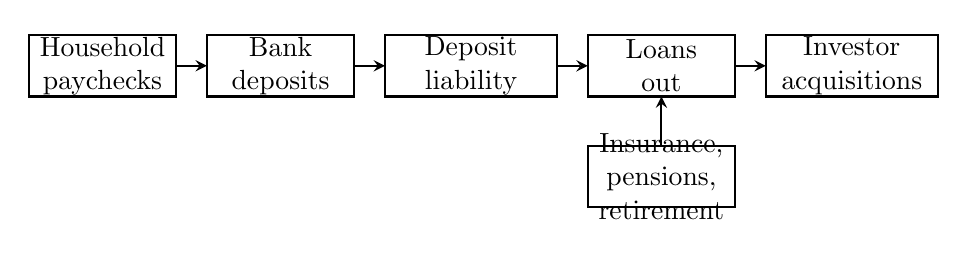
\begin{tikzpicture}[x=1cm,y=1cm,>=stealth,thick,scale=0.78]
\draw (0,0) rectangle (2.4,1) node[pos=.5,align=center]{Household\\paychecks};
\draw (2.9,0) rectangle (5.3,1) node[pos=.5,align=center]{Bank\\deposits};
\draw (5.8,0) rectangle (8.6,1) node[pos=.5,align=center]{Deposit\\liability};
\draw (9.1,0) rectangle (11.5,1) node[pos=.5,align=center]{Loans\\out};
\draw (12.0,0) rectangle (14.8,1) node[pos=.5,align=center]{Investor\\acquisitions};

\draw[->] (2.4,0.5) -- (2.9,0.5);
\draw[->] (5.3,0.5) -- (5.8,0.5);
\draw[->] (8.6,0.5) -- (9.1,0.5);
\draw[->] (11.5,0.5) -- (12.0,0.5);

\draw (9.1,-1.8) rectangle (11.5,-0.8) node[pos=.5,align=center]{Insurance,\\pensions,\\retirement};
\draw[->] (10.3,-0.8) -- (10.3,0);
\end{tikzpicture}
\end{figure}

The point is not moral outrage at finance. The point is structural. Institutions cannot leave deposited household money inert. Their own balance-sheet design drives it back into circulation, where informed borrowers can use it.

\subsection{Question \& Answer}

\paragraph{Question.} Why does saving money fail when inflation outruns the bank?

\paragraph{Answer.} McElroy answers with a standard real-return argument in plain language. If the bank yields one or two percent and inflation is two or three percent, purchasing power erodes.

\begin{align}
r_{\text{bank}} &\approx 1\%\text{--}2\%,\qquad \pi \approx 2\%\text{--}3\%,\\
r_{\text{real}} &\approx r_{\text{bank}} - \pi \in [-2\%,0\%].
\end{align}

This is why he says one cannot save one's way to wealth. The lecture is not claiming that cash reserves are worthless. It is claiming that passive nominal return below inflation is not a serious wealth strategy. McElroy's closing line then returns us to the beginning of his section: find a great mentor who has really done something. The social and the financial arguments remain tied together.

\section{Robert Kiyosaki: Debt, Sales, Rejection, and Anti-School Polemic}

\paragraph{Anecdote.} The final interview is staged as the meeting with the man who ``wrote the book on money.'' The theatrical framing matters, because Kiyosaki does not merely repeat earlier lessons. He hardens them. Where earlier speakers imply, he states. Where earlier speakers soften, he attacks.

\paragraph{Claim.} His first answer is immediate: real estate. He likes real estate because he can use debt. The chapter must preserve the two halves of this claim together. Debt is a tool of enlargement, and debt is a danger.

\subsection{Question \& Answer}

\paragraph{Question.} If debt is dangerous, why does Kiyosaki still call debt money?

\paragraph{Answer.} Because debt enlarges the asset base one can control. In the barest formal reconstruction, we may write

\begin{equation}
A_{\text{acquired}} = E + D_{\text{debt}},
\end{equation}

where \(E\) is one's own equity and \(D_{\text{debt}}\) is borrowed capital. This is the positive side of the doctrine. But Kiyosaki immediately turns to the other side. Debt is like a loaded gun. Used badly, it ruins the borrower. His macro illustration is political and polemical rather than academic. He cites a U.S.\ debt figure above

\begin{equation}
D_{\text{US}} > \$38\,\text{trillion}
\end{equation}

as an example of destructive misuse. We should keep the asymmetry explicit. Debt is not praised because it is safe. It is praised because it is powerful, and therefore requires intelligence.

\paragraph{Mechanism.} Kiyosaki then traces the origin of this view back to his rich-dad teaching. One must first learn to sell. His poor-dad world treated salesmen with contempt. His rich-dad world treated selling as unavoidable. That shift matters because it changes the order of operations. Entrepreneurship, in this account, begins not with product or profession but with the ability to move another mind.

\subsection{Question \& Answer}

\paragraph{Question.} Why is sales treated as prior to entrepreneurship rather than downstream of it?

\paragraph{Answer.} Because Kiyosaki defines sales as communication under resistance. The real obstacle is not technique but rejection. His examples are numerically memorable and structurally useful. He says he asked his future wife out \(50\) times, and he stayed at Xerox until he reached the top sales rank.

\begin{align}
n_{\text{asks}} &= 50,\\
\text{attempt} &\to \text{rejection} \to \text{renewed attempt}.
\end{align}

Each refusal is therefore not a terminal state but a transition rule. The same logic appears in the Xerox story:

\begin{equation}
\operatorname{rank}_{\text{Xerox}} = 1.
\end{equation}

We should not treat this as a universal theorem that only rank one matters everywhere. But within the lecture it functions as an ethic of seriousness. If one is going to learn sales, one should learn it under pressure and with proof.

\paragraph{Anti-school polemic.} From here the interview lands where it had long been heading. School, in Kiyosaki's telling, does not teach money. These are his claims, not neutral textbook statements. He says college is a scam; he says school teaches nothing about money; he says he would first learn to make money and only then decide on a profession. The sequence matters. Earlier speakers had already implied that institutions do not teach operational finance. Kiyosaki makes the complaint explicit and then ties it back to debt, sales, and ranking.

By ending here, the lecture does not introduce a new theme. It sharpens the existing ones. Access, leverage, anti-passivity, and the refusal to be frightened by rejection now appear in their most polemical form.

\section{Summary}

The lecture begins as a hunt for wealthy people and ends as a compact algebra of wealth. First, wealth is concentrated but guarded, so access must be earned under repeated social friction. Second, the move from a \$10 million company to a \$100 million company is a question of structure built before demand, not after it. Third, time is fixed at \(24\) hours, so divergence comes through allocation. Fourth, retained capital compounds when owner draw stays small. Fifth, speed lowers response latency and keeps opportunity from decaying. Sixth, institutional money flows back into credit markets, where informed borrowers can use it. Finally, debt, sales, and rejection are presented not as side skills but as hard operating instruments.

What makes the transcript unusually valuable is that it never floats very long in abstraction. Each doctrine is tied to a person, a number, a cash-flow example, a refusal, or a bottleneck. That is why the notes should preserve the lecture's unfolding rhythm. The host goes looking for rich people. What he gradually finds, and what we gradually write down, is a sequence of rules.